%Class
\documentclass{article}

%Preamble
\usepackage{graphicx}
\usepackage[left=2.5cm, right=2.5cm, top=2cm, bottom=3cm]{geometry}
\usepackage{hyperref}
\usepackage{enumerate}
\usepackage{listings}
\usepackage{xcolor}

\lstdefinestyle{sharpc}{
    language=[Sharp]C,
    frame=lr,
    rulecolor=\color{blue!80!black},
    keywordstyle=\color{blue},
    commentstyle=\color{green!40!black},
    stringstyle=\color{orange},
    basicstyle=\ttfamily\small,
    breaklines=true,
    showstringspaces=false,
    tabsize=4
}


\title{HULK}
\author{Rafael A. Sanchez Martinez \\ Universidad de la Habana \\ Grupo: C-113}
\date{}

\begin{document}

\maketitle

\begin{figure}[h]
    \centering
    
\includegraphics[width=0.5\textwidth]{assets/hulk_logo.jpeg}
    \caption{Havana University Language for Kompilers}
\end{figure}

\newpage
% Define un comando para mostrar y copiar el texto
\newcommand{\copiabletext}[2]{%
    \href{#2}{\texttt{#1}}%
}

\begin{center}
    \centering
    \section{Introduction}
\end{center}
Welcome to the user manual of HULK, the programming language of the University of Havana. This manual is divided into 5 sections, each one dedicated to a part of the interpreter. The first section explains how to install the interpreter, the second section explains how to use the interpreter, the third section explains how to use the lexical analyzer, the fourth section explains how to use the syntax analyzer and the fifth section Explains how to use the expression evaluator.

\subsection{Start}
    \begin{itemize}
        \item To start using the interpreter, you must download the source code of the interpreter from the project's github repository. Once the source code has been downloaded, the project must be run using the `dotnet run' command from a terminal open in the project folder.
        \item Another option is to run the script which will take care of everything
        \item See previous report in \url{https://github.com/ARKye03/mini_kompiler.git}
    \end{itemize}

\begin{figure}[h]
    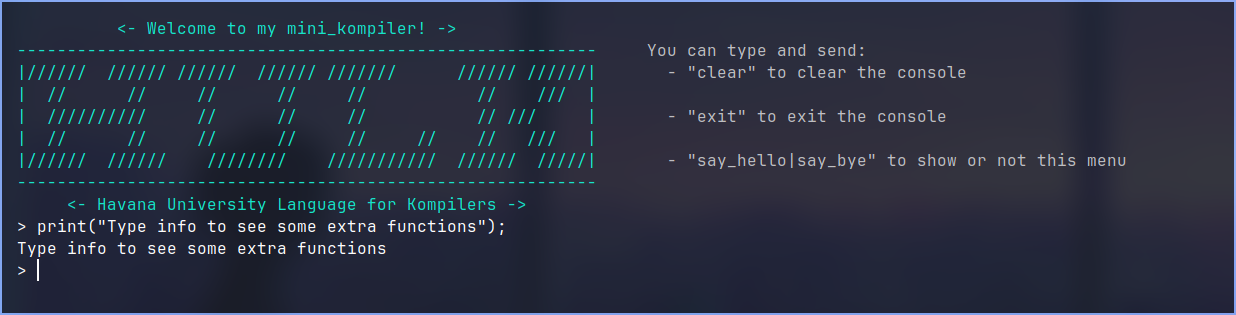
\includegraphics[width=1\textwidth]{assets/hulk_scr.png}
    \caption{Havana University Language for Kompilers}
\end{figure}
    
\subsection{Summary}
HULK (Havana University Language for Compilers) is an educational, type-safe, object-oriented and incremental programming language, designed for the Introduction to Compilers course of the Computer Science degree at the University of Havana.

A simple `Hola Mundo' in HULK looks like this:

    \hbox{print{(`Hola mundo')}}

    From a bird's eye view, HULK is an object-oriented programming language, with simple inheritance, polymorphism, and class-level encapsulation. Additionally, in HULK it is possible to define global functions outside the scope of all classes. It is also possible to define a single global expression that constitutes the entry point to the program.

    Most syntactic constructs in HULK are expressions, including conditional statements and loops. HULK is a statically typed language with optional type inference, meaning that some (or all) parts of a program can be annotated with types and the compiler will check all operations for consistency.

     But, in this case, since it is a project for 1st year students, it is a bit simplified.
     In this case, let's say, we have a one-line interpreter, which allow us, to evaluate expressions like:
     \begin{itemize}
        \item Like I said above, \hbox{print{(``Hello World'')}}
            \begin{itemize}
                \item Which is equivalent to \hbox{$print(``Hello'' + `` World'')$}
                \item And \hbox{print{(``Hello'' @ `` World'')}}
            \end{itemize}
        \item All basics `instructions' can handle simple math expressions like:
            \begin{itemize}
                \item $``2 \pm  5;''$ || $``147.6 \pm  -63;''$
                \item $``8 \times  2;''$ || $``200 \div 3;''$
                \item $``2^{64};''$ || $``sqrt(3969)'' \rightarrow  ``\sqrt{3969}''$ || $``\log(2, 10);''$
                \newpage
                \item Mathematical functions:
                    \begin{itemize}
                        \item[Sin{(x)}:] Returns the sine of x, where x is in radians. Example: Sin{(0)} returns 0.
                        \item[Cos{(x)}:] Returns the cosine of x, where x is in radians. Example: Cos{(0)} returns 1.
                        \item[Tan{(x)}:] Returns the tangent of x, where x is in radians. Example: Tan{(0)} returns 0.
                        \item[Log{(x)}:] Returns the natural logarithm (base 10) of x. Example: Log{(1)} returns 0.
                        \item[Ln{(x)}:] Returns the natural logarithm (base e) of x. Example: Ln{(1)} returns 0.
                        \item[Sqrt{(x)}:] Returns the square root of x. Example: Sqrt{(4)} returns 2.
                        \item[Abs{(x)}:] Returns the absolute value of x. Example: Abs{(-5)} returns 5.
                        \item[Pow{(x, y)}:] Returns x raised to the power of y. Example: Pow{(2, 3)} returns 8.
                        \item[Exp{(x)}:] Returns e raised to the power of x. Example: Exp{(1)} returns approximately 2.71828.
                        \item[Floor{(x)}:] Returns the largest integer less than or equal to x. Example: Floor{(1.5)} returns 1.
                        \item[Ceil{(x)}:] Returns the smallest integer greater than or equal to x. Example: Ceil{(1.5)} returns 2.
                        \item[Round{(x)}:] Rounds x to the nearest integer. Example: Round{(1.5)} returns 2.
                        \item[Rand{(min, max)}:] Returns a random integer between min (inclusive) and max (exclusive). Example: Rand{(10, 20)} returns a random number between 10 and 20.
                        \item[Factorial{(x)}:] Returns the factorial of x. Example: Factorial{(5)} returns 120.
                        \item[Fibonacci{(x)}:] Returns the xth number in the Fibonacci sequence. Example: Fibonacci{(5)} returns 5.
                        \item[IsPrime{(x)}:] Returns true if x is a prime number, false otherwise. Example: IsPrime{(5)} returns true.
                        \item[IsEven{(x)}:] Returns true if x is an even number, false otherwise. Example: IsEven{(5)} returns false.
                        \item[IsDivisible{(x, y)}:] Returns true if x is divisible by y, false otherwise. Example: IsDivisible{(10, 5)} returns true.
                        \item[IsPalindrome{(x)}:] Returns true if x is a palindrome, false otherwise. Example: IsPalindrome{(``radar'')} returns true.
                        \item[Max{(x, y)}:] Returns the maximum of x and y. Example: Max{(2, 3)} returns 3.
                        \item[Min{(x, y)}:] Returns the minimum of x and y. Example: Min{(2, 3)} returns 2.
                    \end{itemize}
                \item And thats pretty much it $\land\times \land$ 
            \end{itemize}
        \item Evaluable expressions are:
            \begin{itemize}
                \item Printing:
                    \begin{description}
                    \item[] This expression keyword receives another expressions as argument, and evaluates it, and print the returned value
                    \item[] $print(55)$; shows 55 || $print(``Kitty'')$; shows Kitty
                    \end{description}
                \item Variables:
                    \begin{description}
                        \item[] This one, contains two important keywords, ``LetKeyword'' and ``InKeyword''.
                        \item[] A basic let-in expression is: ``let $<var\_name>$ in $<statement>$''
                        \item[] Example: ``let x = ${(63 \pm 109)}^2$ in $print{(x)}$; ''
                    \end{description}
                \item Conditions:
                    \begin{description}
                        \item[] Basic and classic conditions:
                        \item[] if (condition) $<do\_if\_true>$ else $<do\_if\_false>$
                        \item[] ``if (1024 \% 2 == 0) $print(``Even'')$ else $print(``Odd'')$; ''
                    \end{description}
                \item Functions:
                    \begin{itemize}
                        \item Declare functions:
                        \begin{description}
                            \item[] To declare functions simple do:
                            \item[] function $function\_name${(arguments)} $=>$ $<statement>$;
                            \item[] Example: function Pow$(x,y)$ $=>$ $x^y$;
                            \item[] This can be used like:
                            \item[] ``let number = $Pow(2,5)$ in $print(number)$; ''
                        \end{description}
                    \end{itemize}
                \item Note: A statement is basically another instruction or expression.
            \end{itemize}
        \newpage
        \item Some expressions can be:
            \begin{enumerate}
                \item print{(``Hello World'')};
                \item print{(($({(1 + 2)} ^ 3)$ * 4) / 5)};
                \item print{($\sin{(2 * PI)}^2$ + $\cos(3 * PI / \log(4, 64))$)};
                \item function $\tan{{(x)}}$ $=>$ $\sin{{(x)}}$ / $\cos{{(x)}}$;
                \item let x = PI/2 in $print(\tan{(x)}$);
                \item let number = 42, text = ``The meaning of life is'' in print{(text @ number)};
                    \begin{itemize}
                        \item let number = 42 in (let text = ``The meaning of life is'' in (print$(text \ @ \ number)$));
                    \end{itemize}
                \item print$(7 + (let \ x = 2 \ in \ x * x))$;
                \item let a = 42 in if (a \% 2 == 0) print$(``Even'')$ else print$(``odd'')$;
                \item let a = 42 in print$(if \ (a \ \% \ 2 == 0)$ ``even'' else ``odd'');
                \item function fib$(n)$ $=>$ if (n $>$ 1) fib$(n-1)$ + fib$(n-2)$ else 1;
            \end{enumerate}
        \item And on and on, use your imagination, except if you are my programming teacher, please don't get creative, I beg you.
     \end{itemize}
\newpage
\section{Analizador Lexico}

\lstset{style=sharpc}
\begin{lstlisting}
    private object power()
    {
        var left = primary();

        while (true)
        {
            var token = lexer.get_next_token();

            if (token.type != TokenType.Operator || token.value != "^")
            {
                lexer.unget_token(token);
                return left;
            }
            var right = primary();
            left = BinaryOperation(left, token, right);
        }
    }
\end{lstlisting}


\newpage
\begin{center}
    \centering
    \section{Interpreter}
\end{center}

\subsection{Parser}

A parser is a program or a component of a program that analyzes a string of symbols according to a set of rules. A parser can be used for different purposes, such as understanding natural language, processing computer languages, or parsing data structures. A parser typically breaks down the input into smaller units called tokens, and then assigns them to categories based on their syntax and semantics. A parser may also produce a representation of the input, such as a parse tree or an abstract syntax tree, that shows the hierarchical structure and the relationships between the tokens.

\subsection{My Parser}

In my case, I handle, 2 types of `expressions', basic statements, and return expressions, the first ones, generally are used to print values, second ones to handle complex operations, you won't even notice them, there are a third type of expression, that derives from the return expressions, used only on declared functions.

My parsing life starts with the Run{()} function, used to parse and execute a series of statements in the source code of a programming language. This is an overview:
\begin{itemize}
\item It first gets the next token from the lexer, using `main' lexer function above explained.
\item If the token is a PrintKeyword, it expects an opening parenthesis `(', evaluates the expression inside the parenthesis, checks for a closing parenthesis `)', and then prints the result of the evaluated expression.
\item If the token is a LetKeyword, it calls the assignment{()} method to process the assignment of values to variables.
\item If the token is an IfKeyword, it calls the Conditional{()} method to process the conditional instruction.
\end{itemize}
Some Statements must be processed, for that there is statement{()}:
\begin{itemize}
    \item Basically does the same as Run{()}, but with extras
    \item If the token is an `Identifier' or `Number', it does nothing.
    \item If the token is an `EOF' (end-of-file), it returns from the method.
    \item If the token is not recognized, it prints an error message.
    \item Finally, it checks if there is a semicolon (end-of-line `EOL' token) and either advances to the next statement or returns the token to the lexer to be analyzed in the next iteration.
\end{itemize}
Let-In expressions are handled with assignment{()} method:
\begin{itemize}
    \item It first gets the next token from the lexer, which should be an identifier (the variable name).
    \item It then expects an equals `=' operator.
    \item It evaluates the expression on the right side of the equals operator to get the assigned value.
    \item It assigns the value to the variable in the variables dictionary.
    \item It then checks if there is a comma, indicating another assignment statement, and recursively calls assignment{()} if there is.
If there is no comma, it expects an in keyword.
Finally, it calls the statement{()} method to execute the next statement.
\end{itemize}

\newpage
Basic conditional statements, processed by Conditional{()}:
\begin{itemize}
    \item It first gets the next token from the lexer, which should be an opening parenthesis `('.
    \item It then evaluates the left-hand side of the comparison, expects a comparison operator, and evaluates the right-hand side of the comparison.
    \item It checks for a closing parenthesis `)'.
    \item It then performs the comparison operation based on the comparison operator and stores the result.
    \item If the comparison result is true, it calls the statement{()} method to execute the next statement.
    \item If the comparison result is false, it skips to the else part of the if-else statement and executes the statement there.
    \item If there is no else part, it prints an error message.
\end{itemize}
Note: RConditional{()} and RConditional{(List<Token> tokens)}, are simple variations of Conditional{()}, used on return expressions and functions return expressions respectively. 

\subsection{Recursive Descent Parser}
The jewel in the crown revolves around these functions, they are what allow everything to flow as well as my programming skills allow.

\begin{itemize}
    \item expression{()}
        \begin{itemize}
            \item It first evaluates a term.
            \item It then enters a loop where it gets the next token from the lexer and checks if it's an operator.
            \item If the operator is @, it evaluates the next term and concatenates it with the left-hand side.
            \item If the operator is + or -, it evaluates the next term and performs the binary operation with the left-hand side and the operator.
            \item If the token is not an operator, it returns the token to the lexer and returns the left-hand side as the result of the expression.
        \end{itemize}
    \item term{()}
        \begin{itemize}
            \item It first evaluates a power.
            \item It then enters a loop where it gets the next token from the lexer and checks if it's a multiplication, division, or modulo operator.
            \item If the token is not one of these operators, it returns the token to the lexer and returns the left-hand side as the result of the term.
            \item If the token is one of these operators, it evaluates the next power and performs the binary operation with the left-hand side and the operator.
        \end{itemize}
    \item power{()}
        \begin{itemize}
            \item It first evaluates a primary expression.
            \item It then enters a loop where it gets the next token from the lexer and checks if it's a power operator (\^).
            \item If the token is not a power operator, it returns the token to the lexer and returns the left-hand side as the result of the power expression.
            \item If the token is a power operator, it evaluates the next primary expression and performs the binary operation with the left-hand side and the operator.
        \end{itemize}
    \item primary{()}
        \begin{itemize}
            \item It first gets the next token from the lexer.
            \item It checks if the token is a function call, and if so, it parses the arguments and calls the function.
            \item If the token is a number, it returns the number.
            \item If the token is a string literal, it returns the string.
            \item If the token is an identifier, it returns the value of the variable with that name.
            \item If the token is an opening parenthesis (, it evaluates the expression inside the parentheses.
            \item If the token is a let keyword, it parses a let-in expression.
            \item If the token is an if keyword, it parses an if-else expression.
            \item If the token is a minus operator -, it negates the next number.
            \item If the token is none of the above, it prints an error message.
        \end{itemize}
\end{itemize}

\texttt{Note:} These functions each have an overload specifically designed to handle expressions within functions. Check fnizer.cs

The function that performs Binary Operations on two operands. Simple overview:
\begin{itemize}
    \item It first checks if the operator token is indeed an operator.
    \item If the operator is +, it adds the operands if they are both floats or concatenates them if they are both strings.
    \item If the operator is -, it subtracts the operands if they are both floats.
    \item If the operator is @, it concatenates the operands if they are both strings.
    \item If the operator is *, it multiplies the operands if they are both floats.
    \item If the operator is \^, it raises the left operand to the power of the right operand if they are both floats.
    \item If the operator is /, it divides the left operand by the right operand if they are both floats.
    \item If the operator is %, it calculates the remainder of the division of the left operand by the right operand if they are both floats.
    \item If the operator is none of the above, it prints an error message.
    \item If the token is not an operator, it prints an error message.
\end{itemize}
An extra encapsulation is ConcatenateValues():
\begin{itemize}
    \item If both operands are strings, it concatenates them.
    \item If one of the operands is a string, it converts the other operand to a string and then concatenates them.
    \item If neither operand is a string, it tries to add them if they are both floats.
    \item If the operands cannot be concatenated or added, it prints an error message.
\end{itemize}
\newpage
\section{Introduction}
This is the report of my compiler project. The compiler is written in C++ and
\newpage
\section{Introduction}
This is the report of my compiler project. The compiler is written in C++ and
\newpage


\end{document}